\documentclass{standalone}
\usepackage{standalone}

\begin{document}

\subsection{Neural Network Design}
A three-layers feed forward supervised network is designed to suit the purpose. The input layers has 27 neurons, taking the 27 extracted features from the previous step. We used 40 neurons in output layer, because it has 40 different output as shown in \ref{table:OutputTypes}. In the hidden layer we have 180 neurons connecting input and output layers (including bias). Figure \ref{fig:PerceptronModel} shows the network design.

\begin{table}
\centering
\caption{The output types of Neural Network}
\label{table:OutputTypes}
\begin{tabular}{|l|r|}
\hline
Output type & Count  \\
\hline
Bangla Digits   & 10 \\
Class letters   & 7  \\
Metropolitan and district words  & 23 \\
\hline
\end{tabular}
\end{table}

\begin{figure}[]
     \centering
     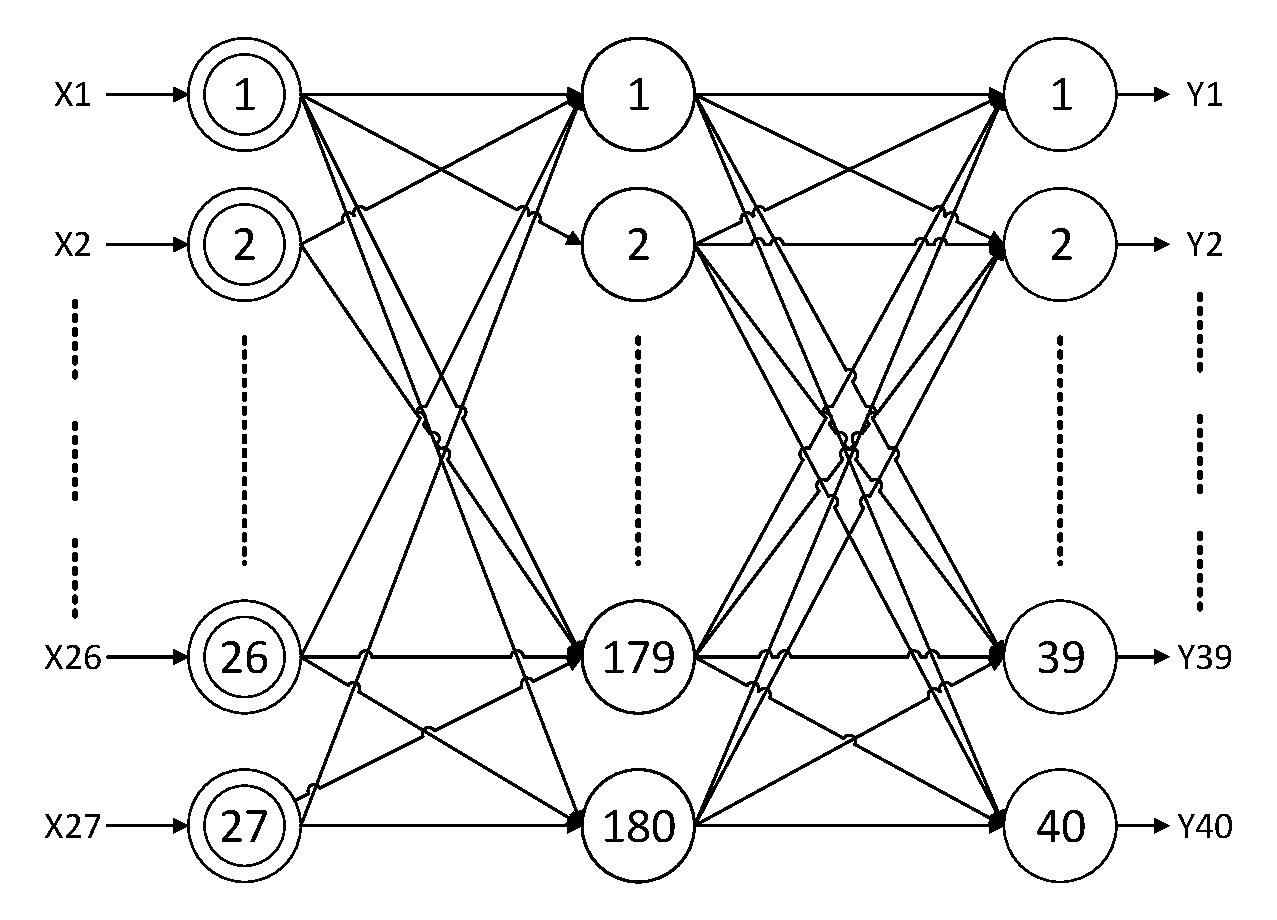
\includegraphics[width=0.8\linewidth]{./img/plots/neural}
     \caption{Design of the Neural Network}
     \label{fig:PerceptronModel}
\end{figure}



\subsection{Training Process}
Due to the diversity and complexity of Bangla letters this stage is very challenging.

\subsubsection{Collecting training data}
The training database should have several images for each set of license plate characters, with the combination of various fonts and positions of the characters. In detected license plate, it is well possible for the characters to be rotated or skewed in more than 15 degrees. We used original character segments from the previous steps and as well as many auto-generated characters with different fonts, angles, and rotation. 

After the training database is collected, we had to convert all of the images into same binary format. And labeled them accordingly. 

\subsection{Recognition}
The input data is converted into 27 column matrix of features before passing to the neural network. Using forward propagation we then calculate the output from the network. Then we convert the output to binary array and use it to calculate a hash value. The hash value is matched against a hash-map to determine the label of the output. If the hash matches any containing hash-key in the hash-map we consider it as a recognized character. 

\subsubsection{Output formatting}
    As final step, we collect all recognize letters and arrange them in the standard format separated by dash and commas. We fill any unrecognized characters with underscore (\_) sign.
    
    If more than several license data is available for the same spot we choose the data with the highest probability of being accurate by analyzing the output matrix.

\end{document}